\documentclass[10pt,a4paper]{article}

\usepackage[spanish,activeacute,es-tabla]{babel}
\usepackage[utf8]{inputenc}
\usepackage{ifthen}
\usepackage{listings}
\usepackage{dsfont}
\usepackage{subcaption}
\usepackage{amsmath}
\usepackage[strict]{changepage}
\usepackage[top=1cm,bottom=2cm,left=1cm,right=1cm]{geometry}%
\usepackage{color}%
\newcommand{\tocarEspacios}{%
	\addtolength{\leftskip}{3em}%
	\setlength{\parindent}{0em}%
}

% Especificacion de procs

\newcommand{\In}{\textsf{in }}
\newcommand{\Out}{\textsf{out }}
\newcommand{\Inout}{\textsf{inout }}

\newcommand{\encabezadoDeProc}[4]{%
	% Ponemos la palabrita problema en tt
	%  \noindent%
	{\normalfont\bfseries\ttfamily proc}%
	% Ponemos el nombre del problema
	\ %
	{\normalfont\ttfamily #2}%
	\
	% Ponemos los parametros
	(#3)%
	\ifthenelse{\equal{#4}{}}{}{%
		% Por ultimo, va el tipo del resultado
		\ : #4}
}

\newenvironment{proc}[4][res]{%
	
	% El parametro 1 (opcional) es el nombre del resultado
	% El parametro 2 es el nombre del problema
	% El parametro 3 son los parametros
	% El parametro 4 es el tipo del resultado
	% Preambulo del ambiente problema
	% Tenemos que definir los comandos requiere, asegura, modifica y aux
	\newcommand{\requiere}[2][]{%
		{\normalfont\bfseries\ttfamily requiere}%
		\ifthenelse{\equal{##1}{}}{}{\ {\normalfont\ttfamily ##1} :}\ %
		\{\ensuremath{##2}\}%
		{\normalfont\bfseries\,\par}%
	}
	\newcommand{\asegura}[2][]{%
		{\normalfont\bfseries\ttfamily asegura}%
		\ifthenelse{\equal{##1}{}}{}{\ {\normalfont\ttfamily ##1} :}\
		\{\ensuremath{##2}\}%
		{\normalfont\bfseries\,\par}%
	}
	\renewcommand{\aux}[4]{%
		{\normalfont\bfseries\ttfamily aux\ }%
		{\normalfont\ttfamily ##1}%
		\ifthenelse{\equal{##2}{}}{}{\ (##2)}\ : ##3\, = \ensuremath{##4}%
		{\normalfont\bfseries\,;\par}%
	}
	\renewcommand{\pred}[3]{%
		{\normalfont\bfseries\ttfamily pred }%
		{\normalfont\ttfamily ##1}%
		\ifthenelse{\equal{##2}{}}{}{\ (##2) }%
		\{%
		\begin{adjustwidth}{+5em}{}
			\ensuremath{##3}
		\end{adjustwidth}
		\}%
		{\normalfont\bfseries\,\par}%
	}
	
	\newcommand{\res}{#1}
	\vspace{1ex}
	\noindent
	\encabezadoDeProc{#1}{#2}{#3}{#4}
	% Abrimos la llave
	\par%
	\tocarEspacios
}
{
	% Cerramos la llave
	\vspace{1ex}
}

\newcommand{\aux}[4]{%
	{\normalfont\bfseries\ttfamily\noindent aux\ }%
	{\normalfont\ttfamily #1}%
	\ifthenelse{\equal{#2}{}}{}{\ (#2)}\ : #3\, = \ensuremath{#4}%
	{\normalfont\bfseries\,;\par}%
}

\newcommand{\pred}[3]{%
	{\normalfont\bfseries\ttfamily\noindent pred }%
	{\normalfont\ttfamily #1}%
	\ifthenelse{\equal{#2}{}}{}{\ (#2) }%
	\{%
	\begin{adjustwidth}{+2em}{}
		\ensuremath{#3}
	\end{adjustwidth}
	\}%
	{\normalfont\bfseries\,\par}%
}

% Tipos

\newcommand{\nat}{\ensuremath{\mathds{N}}}
\newcommand{\ent}{\ensuremath{\mathds{Z}}}
\newcommand{\float}{\ensuremath{\mathds{R}}}
\newcommand{\bool}{\ensuremath{\mathsf{Bool}}}
\newcommand{\cha}{\ensuremath{\mathsf{Char}}}
\newcommand{\str}{\ensuremath{\mathsf{String}}}

% Logica

\newcommand{\True}{\ensuremath{\mathrm{true}}}
\newcommand{\False}{\ensuremath{\mathrm{false}}}
\newcommand{\Then}{\ensuremath{\rightarrow}}
\newcommand{\Iff}{\ensuremath{\leftrightarrow}}
\newcommand{\implica}{\ensuremath{\longrightarrow}}
\newcommand{\IfThenElse}[3]{\ensuremath{\mathsf{if}\ #1\ \mathsf{then}\ #2\ \mathsf{else}\ #3\ \mathsf{fi}}}
\newcommand{\yLuego}{\land _L}
\newcommand{\oLuego}{\lor _L}
\newcommand{\implicaLuego}{\implica _L}

\newcommand{\cuantificador}[5]{%
	\ensuremath{(#2 #3: #4)\ (%
		\ifthenelse{\equal{#1}{unalinea}}{
			#5
		}{
			$ % exiting math mode
			\begin{adjustwidth}{+2em}{}
				$#5$%
			\end{adjustwidth}%
			$ % entering math mode
		}
		)}
}

\newcommand{\existe}[4][]{%
	\cuantificador{#1}{\exists}{#2}{#3}{#4}
}
\newcommand{\paraTodo}[4][]{%
	\cuantificador{#1}{\forall}{#2}{#3}{#4}
}

%listas

\newcommand{\TLista}[1]{\ensuremath{seq \langle #1\rangle}}
\newcommand{\lvacia}{\ensuremath{[\ ]}}
\newcommand{\lv}{\ensuremath{[\ ]}}
\newcommand{\longitud}[1]{\ensuremath{|#1|}}
\newcommand{\cons}[1]{\ensuremath{\mathsf{addFirst}}(#1)}
\newcommand{\indice}[1]{\ensuremath{\mathsf{indice}}(#1)}
\newcommand{\conc}[1]{\ensuremath{\mathsf{concat}}(#1)}
\newcommand{\cab}[1]{\ensuremath{\mathsf{head}}(#1)}
\newcommand{\cola}[1]{\ensuremath{\mathsf{tail}}(#1)}
\newcommand{\sub}[1]{\ensuremath{\mathsf{subseq}}(#1)}
\newcommand{\en}[1]{\ensuremath{\mathsf{en}}(#1)}
\newcommand{\cuenta}[2]{\mathsf{cuenta}\ensuremath{(#1, #2)}}
\newcommand{\suma}[1]{\mathsf{suma}(#1)}
\newcommand{\twodots}{\ensuremath{\mathrm{..}}}
\newcommand{\masmas}{\ensuremath{++}}
\newcommand{\matriz}[1]{\TLista{\TLista{#1}}}
\newcommand{\seqchar}{\TLista{\cha}}

\renewcommand{\lstlistingname}{Código}
\lstset{% general command to set parameter(s)
	language=Java,
	morekeywords={endif, endwhile, skip},
	basewidth={0.47em,0.40em},
	columns=fixed, fontadjust, resetmargins, xrightmargin=5pt, xleftmargin=15pt,
	flexiblecolumns=false, tabsize=4, breaklines, breakatwhitespace=false, extendedchars=true,
	numbers=left, numberstyle=\tiny, stepnumber=1, numbersep=9pt,
	frame=l, framesep=3pt,
	captionpos=b,
}


\usepackage{caratula} % Version modificada para usar las macros de algo1 de ~> https://github.com/bcardiff/dc-tex


\titulo{Trabajo practico 1}
\subtitulo{Especificacion y Weakest Precondition}

\fecha{\today}

\materia{Algoritmos y Estructura de Datos}
\grupo{Grupo HIBTAYIGAFWKBCHZLZPJ}

\integrante{Dominguez, Mateo Felipe}{924/23}{matedominguez2@gmail.com}
\integrante{Apellido, Nombre2}{002/01}{email2@dominio.com}
\integrante{Apellido, Nombre3}{003/01}{email3@dominio.com}
\integrante{Apellido, Nombre4}{004/01}{email4@dominio.com}

% Declaramos donde van a estar las figuras
% No es obligatorio, pero suele ser comodo
\graphicspath{{../static/}}

\begin{document}

\maketitle

%Y se pueden citar ecuaciones con \verb|\eqref{nombreDeEq}|: \eqref{eq:1}

Ejemplo de itemizado:

\begin{itemize}
	\item Item 1
	\item Item 2
	\item Item 3
\end{itemize}

Ejemplo de enumerado con menor distancia entre items:

\begin{enumerate} \setlength\itemsep{0cm}
	\item Item 1
	\item Item 2
	\item Item 3
\end{enumerate}

Podemos escribir mucho texto. Mucho texto. Mucho texto. Mucho texto. Mucho texto. Mucho texto. Mucho texto. Mucho texto. Mucho texto. Mucho texto. Mucho texto.

Otro párrafo. Otro párrafo. Otro párrafo. Otro párrafo. Otro párrafo. Otro párrafo. Otro párrafo. Otro párrafo. Otro párrafo. Otro párrafo. Otro párrafo. Otro párrafo. Otro párrafo.

\vspace{0.3cm}

Le agregamos una separación entre párrafos. Le agregamos una separación entre párrafos. Le agregamos una separación entre párrafos. Le agregamos una separación entre párrafos. Le agregamos una separación entre párrafos.

\vspace{0.3cm}

%La tabla \ref{tab:ejemplo} es un ejemplo de cómo se hace una tabla.

\begin{table}[h!]
	\centering
	\begin{tabular}{||l c c r||} 
		\hline
		Col1 & Col2 & Col2 & Col3 \\ [0.5ex] 
		\hline\hline
		1 & 6 & 87837 & 787 \\ 
		2 & 7 & 78 & 5415 \\
		3 & 545 & 778 & 7507 \\
		4 & 545 & 18744 & 7560 \\
		5 & 88 & 788 & 6344 \\
		\hline
	\end{tabular}
	\caption{Ejemplo de tabla}
	\label{tab:ejemplo}
\end{table}


%La figura \ref{fig:subfigs} es un ejemplo de cómo se agrega una imagen.

\begin{figure}[ht]
	\centering
	
\includegraphics[width=0.6\textwidth]{logo_dc.jpg}
	\caption{Ejemplo de figura}
	\label{fig:ejemplo}
\end{figure}

\begin{figure}[ht!]
	\begin{subfigure}{0.5\textwidth}
		
\includegraphics[width=0.9\linewidth]{LaTeX-project} 
		\caption{Logo de LaTeX}
		\label{fig:subfig1}
	\end{subfigure}
	\begin{subfigure}{0.5\textwidth}
		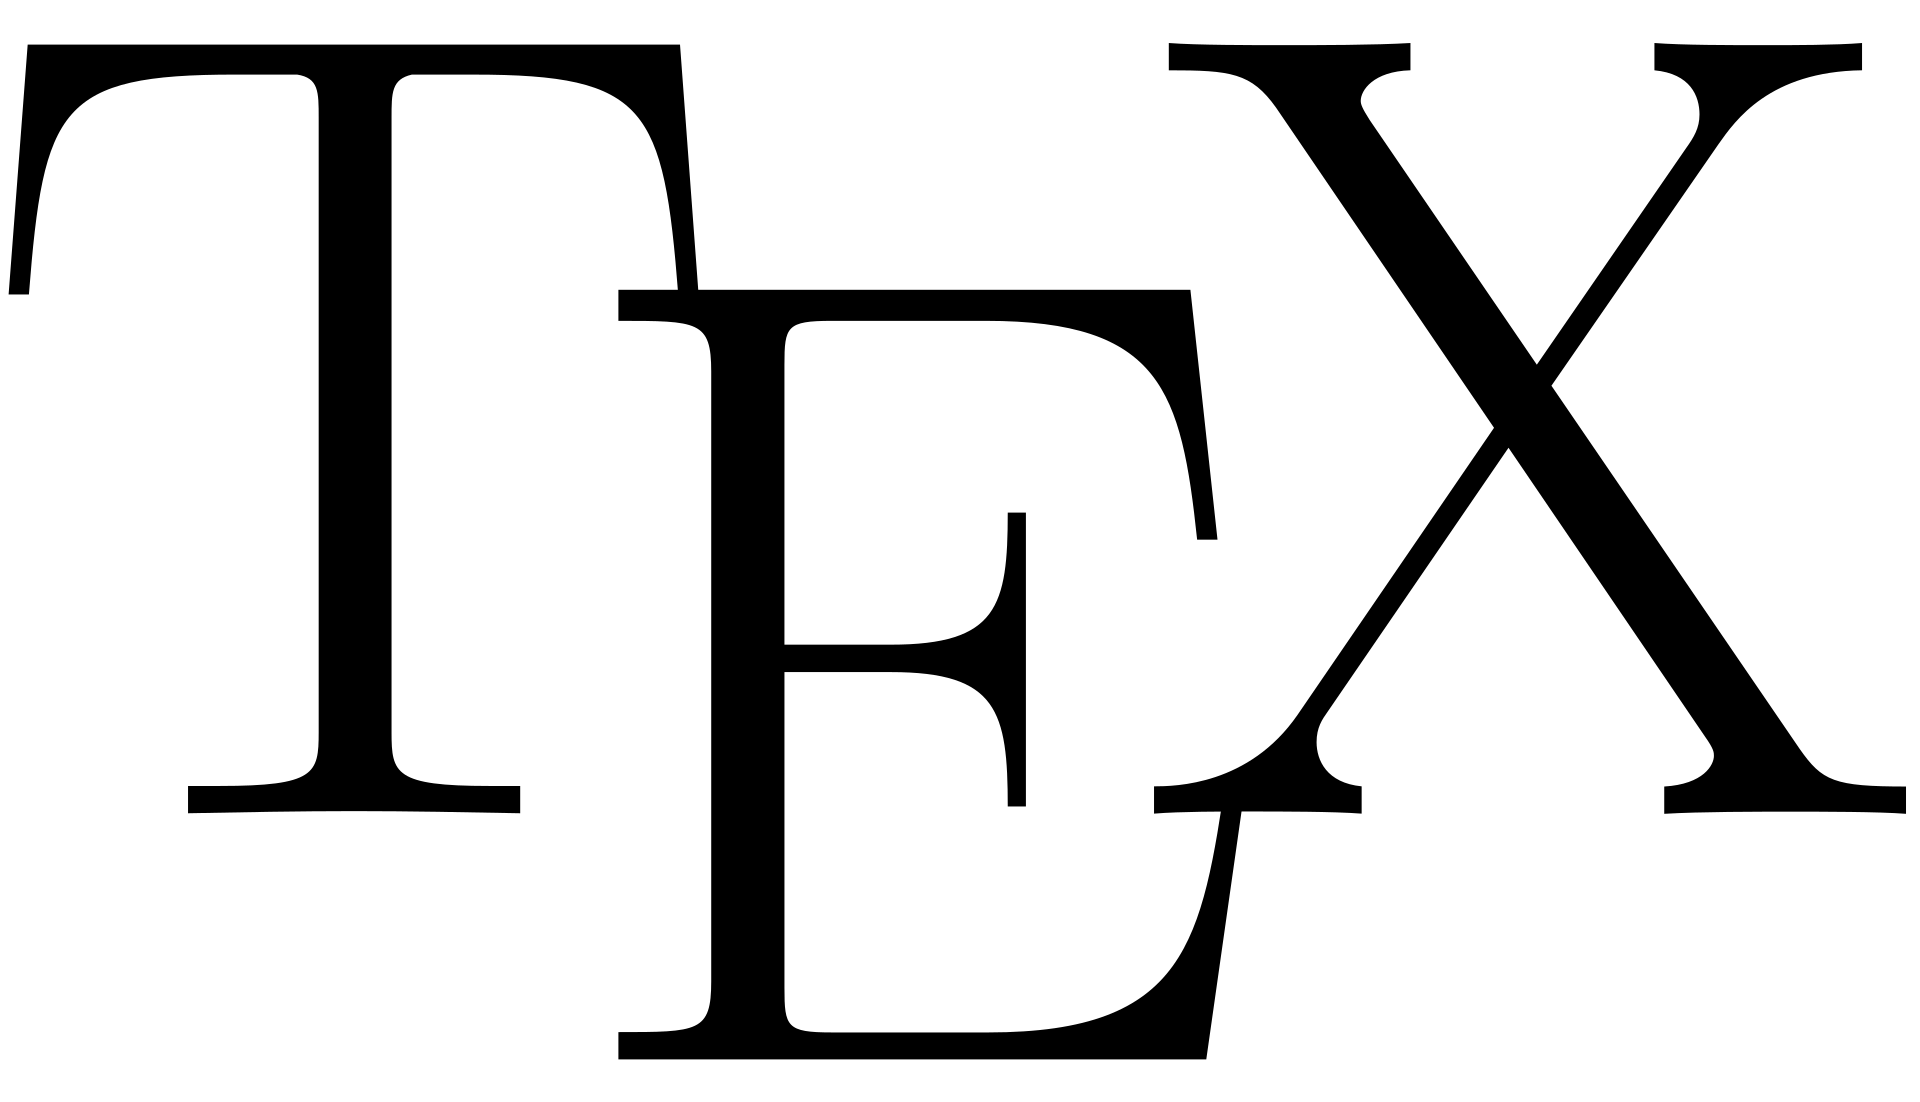
\includegraphics[width=0.7\linewidth]{TeX}
		\caption{Logo de TeX}
		\label{fig:subfig2}
	\end{subfigure}
	%\caption{Ejemplo para poner dos figuras juntas. Y citarlas por separado a (\subref{fig:subfig1}) y (\subref{fig:subfig2}).}
	% OJO: el caption siempre va antes del label
	\label{fig:subfigs}
\end{figure}



% Para hacer que quede todo en una misma linea, se puede usar minipage

%Si se pone un label al \verb|lstlisting|, se puede referenciar: Código \ref{code:for}.

% Punto 1
\section{Especificacion}

% Especificacion punto 1.1
\subsection{grandesCiudades}
\begin{proc}{grandesCiudades}{\In ciudades: \TLista{Ciudad}}{\TLista{Ciudad}}
	\requiere{\neg ciudadesRepetidas(ciudades)}
	\asegura{\neg ciudadesRepetidas(res) \wedge (\forall i : \ent)(0 \leq i < |res| \implicaLuego res[i] \in ciudades \wedge res[i][1] > 50.000)}
\end{proc}

\vspace{0.3cm}

\pred{ciudadesRepetidas}{s: \TLista{Ciudad}}{(\forall i : \ent)(0 \leq i < |s| \implicaLuego (\exists j : \ent)(0 \leq j < |s| \wedge i \neq j \yLuego s[i] = s[j]))}

\vspace{0.3cm}

% Especificaion punto 1.2
\subsection{sumaDeHabitantes}
\begin{proc}{sumaDeHabitantes}{\In menoresDeCiudades: \TLista{Ciudad}, \In mayoresDeCiudades: \TLista{Ciudad}}{\TLista{Ciudad}}
	\requiere{\neg ciudadesRepetidas(menoresDeCiudades) \wedge \neg ciudadesRepetidas(mayoresDeCiudades)}
	\requiere{mismasCiudades(menoresDeCiudades, mayoresDeCiudades)}
	\asegura{|res| = |s_1|}
	\asegura{\neg ciudadesRepetidas(res)}
	\asegura{(\forall i,j : \ent)(0 \leq i,j < |menoresDeCiudades| \yLuego menoresDeCiudades[i][0] = mayoresDeCiudades[j][0] \implicaLuego (res[i][1] = menoresDeCiudades[i][1] + mayoresDeCiudades[j][1])))}
\end{proc}

\vspace{0.3cm}

\pred{mismasCiudades}{s: \TLista{Ciudad}, t: \TLista{Ciudad}}{(\forall i : \ent)(0 \leq i < |s_1| \implicaLuego (\exists j : \ent)(0 \leq j < |s_2| \yLuego s_1[i][0] = s_2[j][0]))}

\vspace{0.3cm}

% Especificacion punto 1.3
\subsection{hayCamino}
\begin{proc}{hayCamino}{\In distancias: \TLista{\TLista{\ent}}, \In desde: \ent, \In hasta: \ent}{Bool}
	\requiere{esCuadrada(distancias)}
	\requiere{(\forall i,j : \ent)(0 \leq i,j < |s| \implicaLuego s[i][j] = s[j][i] \wedge s[i][j] \geq 0)}
	\requiere{0 \leq desde,hasta < |distancias|}
	\asegura{res = True \iff (\exists t : \TLista{\ent})(esCamino(distancias, t, desde, hasta))}
\end{proc}

\vspace{0.3cm}

\pred{esCuadrada}{A : \TLista{\TLista{\ent}}}{(\forall i : \ent)(0 \leq i < |A| \implicaLuego |A[i]| = |A|)}
\vspace{0.1cm}
\pred{esCamino}{s: \TLista{\TLista{\ent}}, t: \TLista{\ent}, n: \ent, m: \ent}{(2 \leq |t| \leq |s| \wedge t[0] = n \wedge t[|t|-1] = m \wedge (\forall i : \ent)(0 \leq i < |t|-1 \implicaLuego 0 \leq t[i] < |s| \wedge s[t[i]][t[i+1]] > 0))}

\vspace{0.3cm}

% Especificaion punto 1.4
\subsection{cantidadCaminosNSaltos}
\begin{proc}{cantidadCaminosNSaltos}{\Inout conexion: \TLista{\TLista{\ent}}, \In n: \ent}{}
	\requiere{conexion = C_0}
	\requiere{esCuadrada(C_0)}
	\requiere{(\forall i,j : \ent)(0 \leq i,j < |C_0|\implicaLuego(C_0[i][j] = C_0[j][i]\wedge(C_0[i][j] = 0 \vee C_0[i][j] = 1)))}
	\requiere{(\forall i,j : \ent)(((0 \leq i,j < |C_0|)\wedge(i = j))\implicaLuego(C_0[i][j] = 0))}
	\requiere{n \geq 1}
	\asegura{|conexion| = |C_0|}
	\asegura{(\forall i,j : \ent)(0 \leq i,j < |conexion| \implicaLuego conexion[i][j] = conexion[j][i])}
	\asegura{(\exists t : \TLista{\TLista{\TLista{\ent}}})(|t| = n \wedge t[0] = C_0 \wedge (\forall i,j : \ent)(0 \leq i < |t| - 1 \wedge 0 \leq j < |t| \implicaLuego |t[i]|=|t[j]| \wedge \\ esCuadrada(t[j]) \wedge APorBEsC(t[i], C_0, t[i+1])) \wedge conexion = t[n-1])}
\end{proc}

\vspace{0.3cm}

\pred{APorBEsC}{A : \TLista{\TLista{\ent}}, B : \TLista{\TLista{\ent}}, C : \TLista{\TLista{\ent}}}{(\forall i,j : \ent)(0 \leq i,j < |C| \implicaLuego (C[i][j] = \sum\limits_{k=0}^{|C| - 1} A[i][k]*B[k][j]))}

\vspace{0.3cm}

% Especificacion punto 1.5
\subsection{caminoMinimo}
\begin{proc}{caminoMinimo}{\In origen: \ent, \In destino: \ent, \In distancias: \TLista{\TLista{\ent}}}{\TLista{\ent}}
	\requiere{esCuadrada(distancias)}
	\requiere{(\forall i,j : \ent)(0 \leq i,j < |s| \implicaLuego s[i][j] = s[j][i] \wedge s[i][j] \geq 0)}
	\requiere{0 \leq origen,destino < |distancias|}
	\asegura{res = \ensuremath{\langle\rangle} \iff \neg conectadas(distancias, origen, hasta)}
	\asegura{esCamino(distancias, res, origen, destino) \wedge esMinimo(distancias, res, origen, destino)}
\end{proc}

\vspace{0.3cm}

\pred{esMinimo}{s: \TLista{\TLista{\ent}}, t: \TLista{\ent}, n: \ent, m: \ent}{(\forall w: \TLista{\ent})(esCamino(s, w, n, m) \implicaLuego sumaDistancias(s,t) \leq sumaDistancias(s,w))}
\aux{sumaDistancias}{s: \TLista{\TLista{\ent}}, t: \TLista{\ent}}{\ent}{\sum\limits_{i=0}^{|t| - 2} s[t[i]][t[i+1]]}

% Punto 2
\section{Demostraciones de correctitud}

% Demostracion punto 2.1
\subsection{Demostrar que la implementacion es correcta con respecto a la especificacion}
\begin{lstlisting}[label=implementacion-punto2]
	res = 0
	i = 0
	while (i < ciudades.length) do
		res = res + ciudades[i].habitantes
		i = i + 1
	endwhile
\end{lstlisting}

\vspace{0.3cm}

\textbf{Demostrar \{P\}S\{Q\}}

\vspace{0.1cm}

\noindent Supongamos ciudades = [(a,10),(b,15)]

\begin{table}[h!]
	\begin{tabular}{| l | l | l |} 
		\hline
		Iteracion & i & res  \\ [0.5ex] 
		\hline
		0 & 0 & 0 \\ 
		1 & 1 & 10 \\
		2 & 2 & 10+15=25 \\
		\hline
	\end{tabular}
	\captionsetup{singlelinecheck=off}
	\caption{Tabla de iteracion}
	\label{tab:iteracion}
\end{table}

$I \equiv 0 \leq i \leq |ciudades| \wedge res = \sum\limits_{j=0}^{i-1} ciudades[j].habitantes$

$ P_c \equiv \{res = 0 \wedge i = 0\}$

$ Q_c \equiv \{res = \sum\limits_{i=0}^{|c|-1} ciudades[i].habitantes\}$

$ B = i < |ciudades|$

\vspace{0.5cm}

\textbf{Paso 1}

\vspace{0.1cm}

\noindent$P_c \implies I ? \\ res = 0 \wedge i = 0 \implies 0 \leq i < |ciudades| \wedge res = \sum\limits_{j=0}^{i-1} ciudades[j].habitantes$

Analizamos variable a variable: \\ $\bullet \ i = 0 \implies 0 \leq i < |ciudades| \\ \bullet \ res = \sum\limits_{j=0}^{i-1} ciudades[j].habitantes = \sum\limits_{j=0}^{-1} ciudades[j].habitantes = 0 \implies res = 0$

\vspace{0.5cm}

\textbf{Paso 2}

\vspace{0.1cm}

\noindent$\{I \wedge B\} S \{I\} \\ \{I \wedge B\} \implies wp(S,I)$

\noindent$\bullet \ \{I \wedge B\} = \{0 \leq i < |ciudades| \wedge \sum\limits_{j=0}^{i-1} ciudades[j].habitantes\} \\ \bullet \ wp(S_1;S_2,I) = wp(S_1,wp(S_2,I))$

\noindent$wp(S_2,I) = wp(i := i + i, 0 \leq i \leq |ciudades| \wedge res = \sum\limits_{j=0}^{i-1} ciudades[j].habitantes) \equiv \\ def(i+1) \yLuego 0 \leq i+1 \leq |ciudades| \wedge res = \sum\limits_{j=0}^{i-1} ciudades[j].habitantes \equiv \\ 0 \leq i+1 \leq |ciudades| \wedge res = \sum\limits_{j=0}^{i-1} ciudades[j].habitantes$

\vspace{0.5cm}

\noindent$wp(S_1,wp(S_2,I)) \equiv wp(res := res + ciudades[i].habitantes, 0 \leq i+1 \leq |ciudades| \wedge res = \sum\limits_{j=0}^{i-1} ciudades[j].habitantes) \equiv \\ def(ciudades) \wedge def(ciudades[i].habitantes) \yLuego 0 \leq i+1 \leq |ciudades| \wedge 0 \leq i+1 \leq |ciudades| \wedge res = \sum\limits_{j=0}^{i-1} ciudades[j].habitantes \equiv \\ 0 \leq i < |ciudades| \yLuego 0 \leq i+1 \leq |ciudades| \wedge 0 \leq i+1 \leq |ciudades| \wedge res = \sum\limits_{j=0}^{i-1} ciudades[j].habitantes \equiv \\ 0 \leq i \leq |ciudades| - 1 \wedge res = \sum\limits_{j=0}^{i-1} ciudades[j].habitantes \equiv \\ 0 \leq i \leq |ciudades| - 1 \wedge res + ciudades[i].habitantes = \sum\limits_{j=0}^{i} ciudades[j].habitantes$

%\aux{auxiliarSuelto}{parametros}{tipoRes}{expresion}
% \paraTodo{variable}{tipo}{expresion}
% \existe{variable}{tipo}{expresion}
% Pueden tener [unalinea] para que no se divida en varias lineas
%\pred{predSuelto}{parametros}{\paraTodo[unalinea]{variable}{tipo}{algo \implicaLuego expresion}}
%\pred{predSuelto}{parametros}{\existe[unalinea]{variable}{tipo}{algo \yLuego expresion}}

\end{document}
